\subsection{センサネットワーク展開時のグループ化}
センサネットワークが展開される初回起動時にグループを作成する手法を述べる.GWノードがセンサノードのトポロジを把握するため,各ノードが周囲のノード情報を探索する.下記にシーケンス図\ref{fig:group_on_activation}を示す.

\begin{enumerate}
    \item グループを構築するに当たり,GWノードに現在のWSNトポロジを通知する必要がある.そのため,センサノード起動時に,BLEにて自身の情報を発信し,同時に周囲のセンサノード情報を収集する.近傍センサノードのリストを作成した後,GWノードへ送信する.
    \item センサノードはリスト送信後,GWノードからグループ構成の通知が来るまでLoRaWANにて通信を行う.
    \item GWノードがセンサノード情報を集約した後,センサノードの固有ID,及び個々の信号強度を用いて重複ノードのないグループを作成しグループごとに1つGLノードを選出する.センサノードがLoRaWANにて次に接続した場合,Downlinkでグループ構成を通知しシーケンスは終了する.
\end{enumerate}

\begin{figure}[]
    \begin{center}
    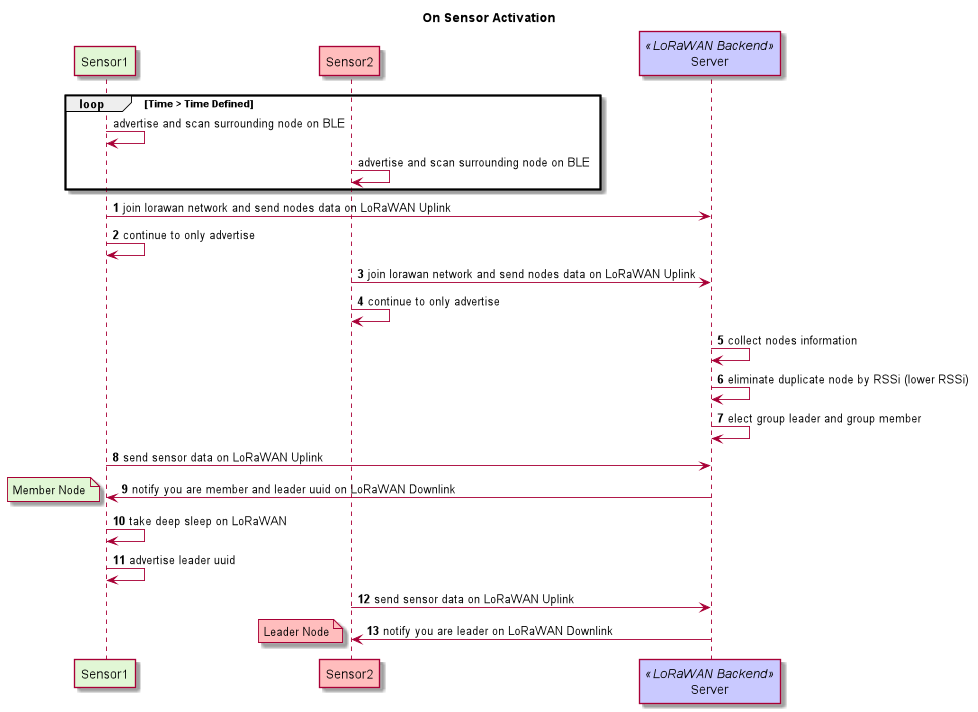
\includegraphics[width=14cm]{figures/グループ化_センサ起動時.png}
    \caption{グループ化の通信方式}
    \label{fig:group_on_activation}
    \end{center}
\end{figure}